\chapter{Observational Health Data Sciences and Informatics (OHDSI)}\label{cap:05OHDSI}

Este capítulo presenta el marco teórico sobre OHDSI y se divide en cuatro secciones:  %\ref{sec:05intro} Introducción y contenidos del capítulo,  
\ref{sec:05OHDSI} ¿Qué es OHDSI?, \ref{sec:05omop} ¿Qué es OMOP? \ref{sec:05Evidencia} ¿Cómo generar evidencia? y \ref{sec:05conclusion} Conclusión.

\section{Introducción} \label{sec:05intro}
%El objetivo es dar a concoer todos los conceptos teóricos de OHDSI y ATLAS. Quién quiera utilizar ATLAS debe conocer OHDSI, debe conocer el CDM, el Vocab, otras herramientas... Son conceptos fundamentales.

La organización Observational Health Data Science and Informatics (OHDSI) es muy importante para el TFG por ser la proveedora de la herramienta de análisis ATLAS, núcleo central del trabajo, y por la relevancia que ha adquirido a nivel europeo en los últimos años.

Por tanto, en este capítulo se pretende dar a conocer al lector el ecosistema completo de la organización que provee la herramienta, en cuanto a los aspectos más generales como los más específicos. \textbf{No se puede entender ATLAS sin entender OHDSI porque las herramientas no están aisladas sino que forman parte de un ecosistema dependiente entre sí}. Todas estas dependencias y conceptos necesarios se exponen en este capítulo para generar un conocimiento profundo subyacente al caso práctico (véase \ref{cap:09caso} ''Caso práctico'') y para poder volver a estos conceptos básicos cuando fuere necesario.

\section{¿Qué es OHDSI?} \label{sec:05OHDSI}

OHDSI, pronunciado en inglés ''Odyseey'', son las siglas de \textit{Observational Health Data Science and Informatics}. OHDSI es una organización colaborativa de ciencia abierta cuyo propósito, de forma muy resumida, es mejorar la investigación cientifico-sanitaria a través de la ciencia de datos y la informática clínica. No obstante, no es solo una organización, sino una comunidad global abierta a todo el que esté interesado y alineado con su misión, visión y objetivos. 

La comunidad se asigna por tanto la misión de ''mejorar la salud empoderando a una comunidad para generar de manera colaborativa evidencia que promueva mejores decisiones de salud y una mejor atención'', y comparte la visión de ''un mundo en el que la investigación observacional produzca una comprensión integral de la salud y la enfermedad'' \cite{OHDSIwebsite}\cite{OHDSIbook}. 

Por otra parte, en El Libro de OHDSI la organización se define así misma como ''una comunidad de ciencia abierta que tiene como objetivo mejorar la salud empoderando a la comunidad para generar de manera colaborativa evidencia que promueva mejores decisiones de salud y mejor atención'' \cite{OHDSIbook}. %La web oficial presenta otra definición algo diferente, se presenta como ''una colaboración de ciencia abierta, interdisciplinaria y de múltiples partes interesadas para resaltar el valor de los datos de salud a través de análisis a gran escala'' \cite{OHDSIwebsite}.

\begin{figure}[H]
    \centering
    
\includegraphics[width=0.90\textwidth]{figures/OHDSIbanner.png}
    \caption{Banner de OHDSI. Extraído de web oficial \cite{OHDSIwebsite}}
    \label{fig:OHDSIbanner}
\end{figure}

Por tanto, a la pregunta sobre \textit{qué es OHDSI} se puede responder apoyándose en cuatro características fundamentales: (i)  una comunidad o red colaborativa, (ii) de ciencia abierta, (iii) estandarizada y (iv) con la finalidad de promover la extracción de evidencia a partir de datos clínicos.

\begin{enumerate}[label=\roman*.]
    \item \textbf{Una comunidad o red colaborativa}. La organización es una comunidad, es decir, se presenta abierta a la incorporación de todo aquel que esté comprometido con su misión. Además se muestra siempre abierta e interesada en la incorporación de nuevos colaboradores, lo que muestran constantemente con el eslogan \textit{''Join the Journey''}, en español, ''únete a la aventura'' (véase Figura \ref{fig:joinTheJourney} ''\textit{Join the Journey}''). Además la organización distribuye a sus colaboradores en nodos por países y en grupos de trabajo según los diferentes componentes de OHDSI. 
    
\begin{figure}[H]
    \centering
    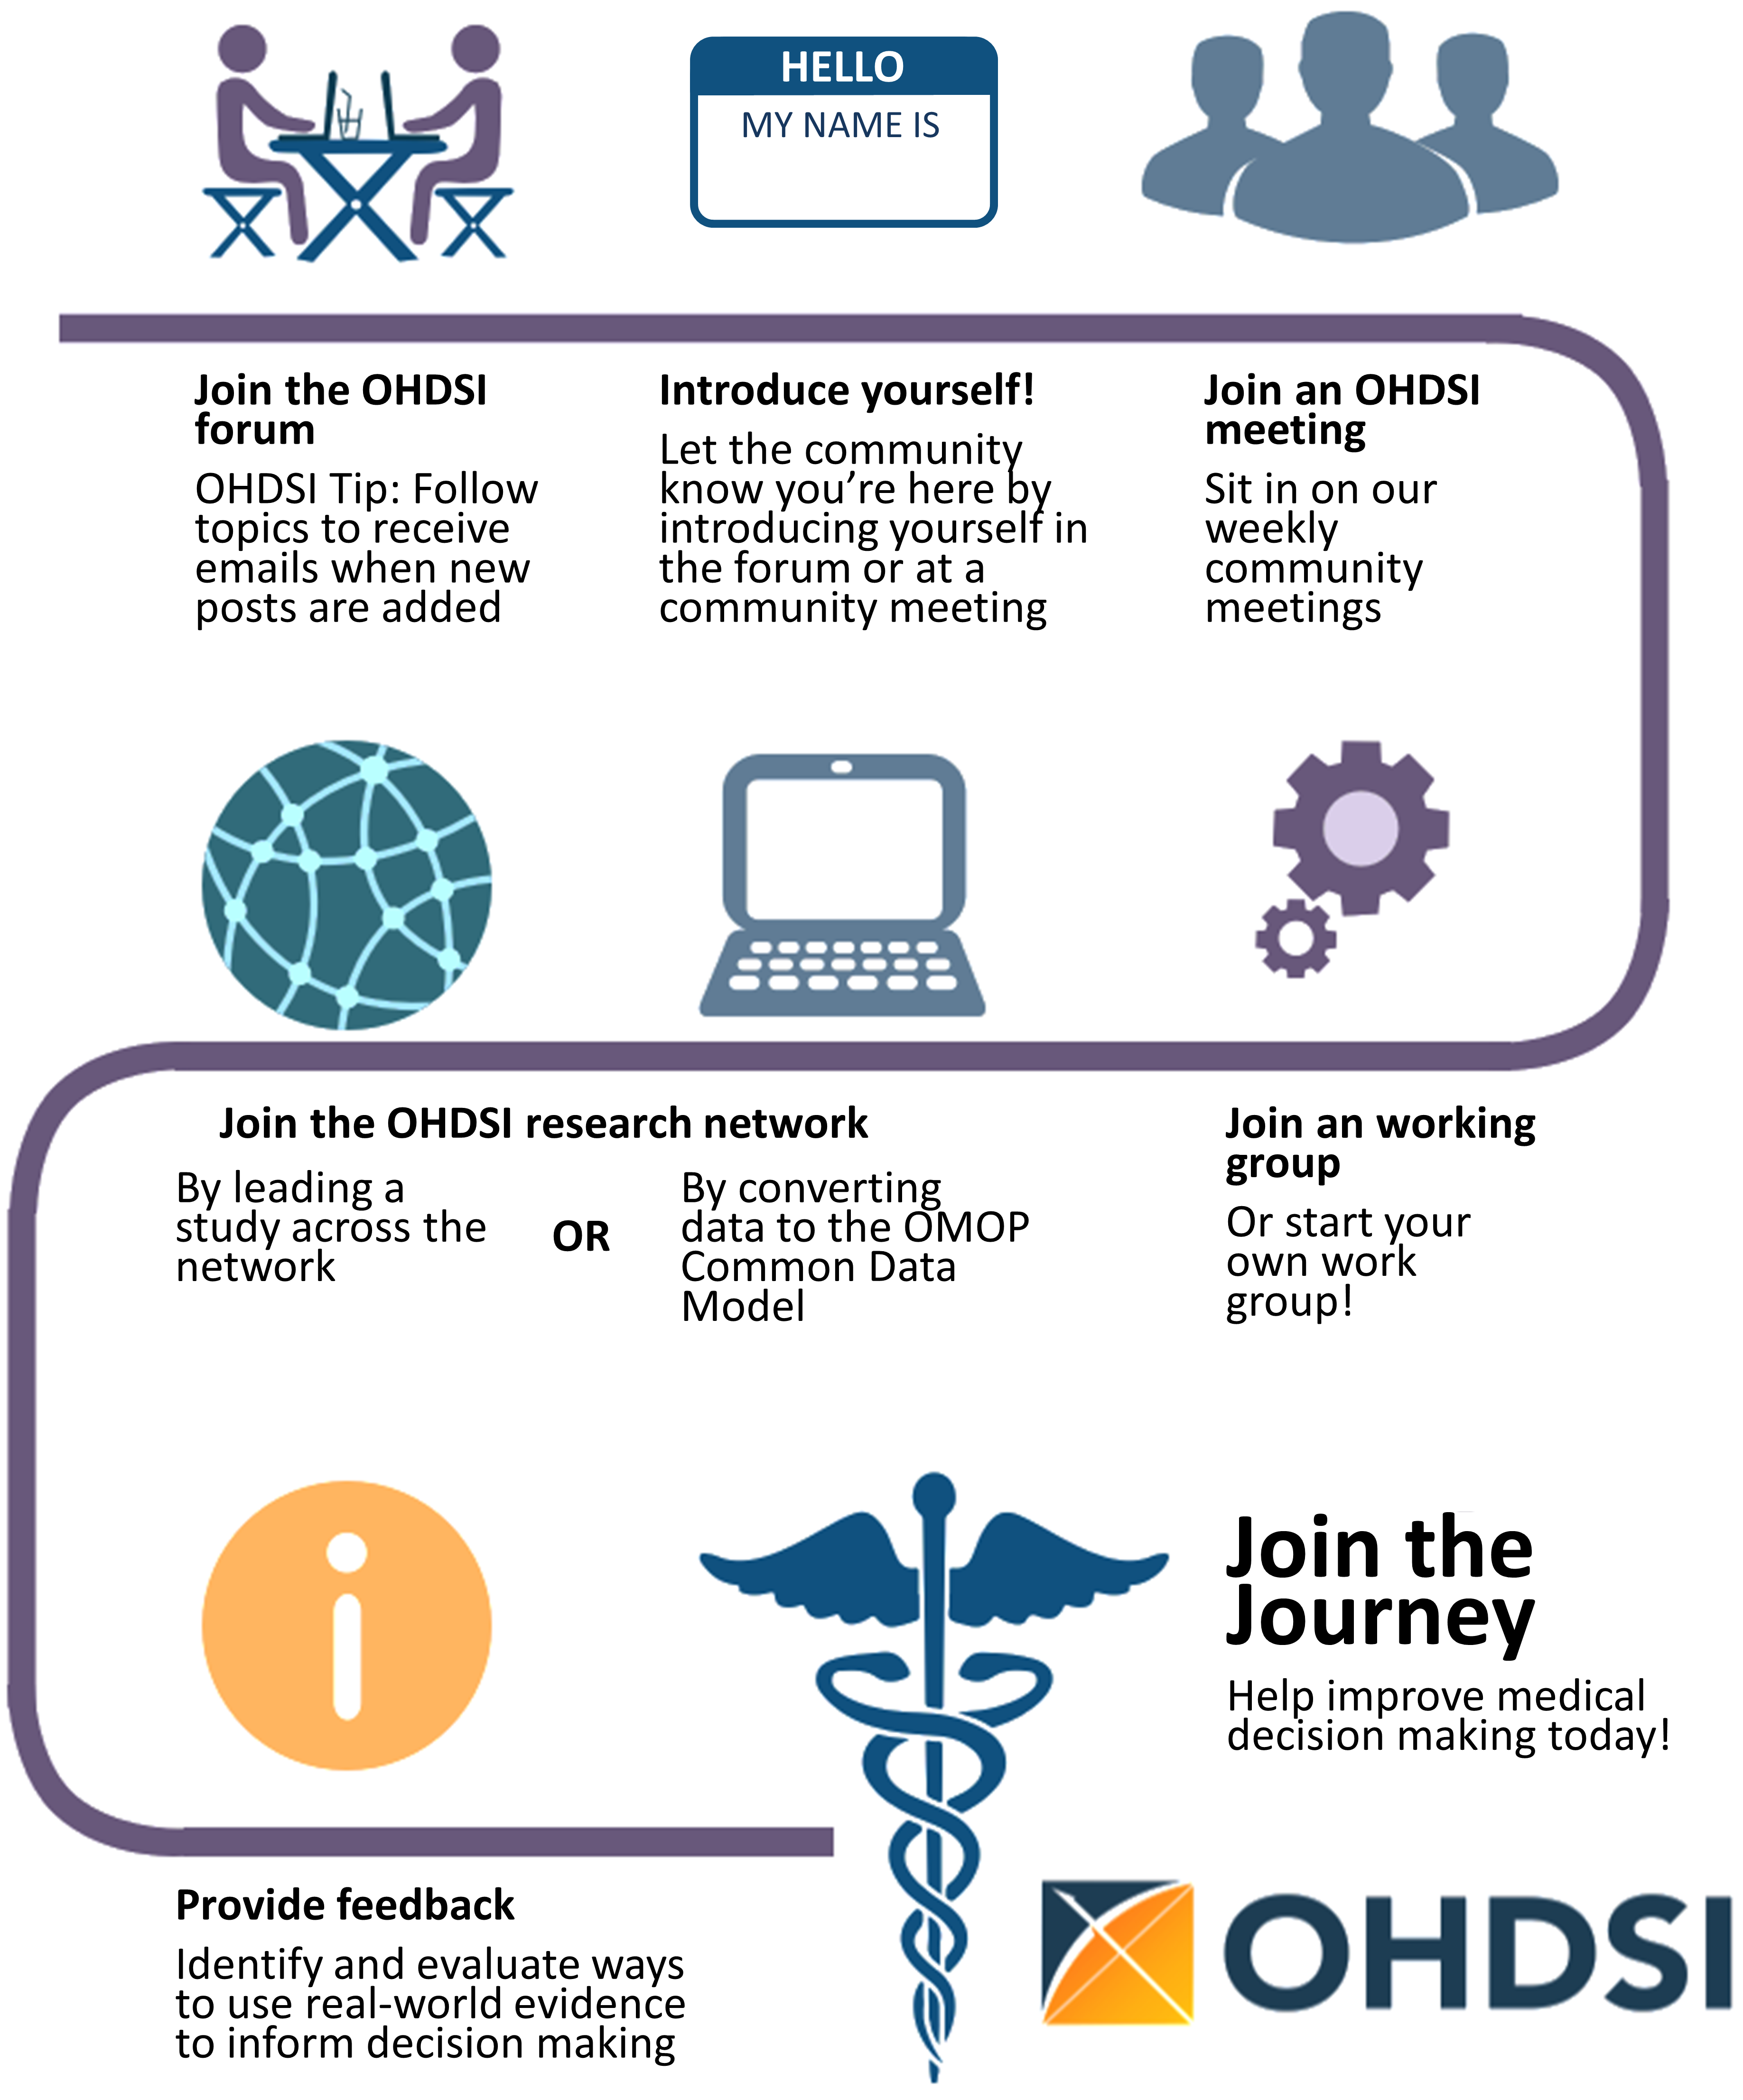
\includegraphics[width=0.50\textwidth]{figures/joinTheJourney.png}
     \caption{\textit{Join the Journey}. Extraído del Libro de OHDSI \cite{OHDSIbook}}
    \label{fig:joinTheJourney}
\end{figure}
    
    %Esta red de colaboradores busca componerse de un gran equipo multidisciplinar, pues se entiende que el propósito que persigue la organización es tan extenso y complejo que es complicado que una única persona albergue todo el conocimiento técnico para desarrollar a la perfección cada etapa de un proyecto, por ello hace especial hincapié en recibir colaboradores expertos en diferentes materias pero que contribuyan al proyecto común de OHDSI.

    \item \textbf{Ciencia abierta}. La forma de trabajar de la organización es muy importante, puesto que promueve la colaboración entre las organziaciones y la participación a través de la ciencia abierta.

    Todos los eventos, publicaciones, herramientas y documentación que elabora OHDSI están disponibles públicamente y de forma gratuita en internet, para que pueda unirse quien quiera (en el caso de los eventos) o consultarse y usarse en cualquier momento (en caso de las herramientas e información). Las dos vías de información por excelencia sobre OHDSI son su página web \cite{OHDSIwebsite} y el \textit{Libro de OHDSI} \cite{OHDSIbook}. Otras vías de información son a través de publicaciones científicas \cite{OHDSIpublications}, tutoriales para principiantes, grabaciones de las reuniones semanales de la comunidad o las conferencias anuales a través de su canal de youtube \cite{OHDSIyt}, canales de mensajería abierta como discord \cite{OHDSIdiscordInvitation} o MS Teams \cite{OHDSIofficeForm}, cientos de repositorios de github con información técnica de cada herramienta \cite{OHDSIgithub} y los foros de la comunidad para solventar dudas y preguntas \cite{OHDSIforums}, entre otros.

    Además, OHDSI asegura la fiabilidad, accesibilidad, interoperabilidad y reproducibilidad de sus estudios a través del cumplimiento de los principios FAIR, que desarrolla en gran extensión en la sección 3.7 de su libro \cite{OHDSIbook}.

    \item \textbf{Estandarización}. OHDSI aboga por estandarizar los modelos de datos y la metodología de la investigación médica a un modelo común, con la finalidad de aumentar la interoperabilidad entre los sistemas y organizaciones sanitarias a nivel mundial.
    
    Esta idea se presenta en el Symposium de 2023 con un ejemplo muy intuitivo: la conexión a la corriente eléctrica a través de una plancha. La conexión de la plancha sería la realización de un estudio sobre unos datos, que serían el enchufe a la corriente eléctrica, siendo el objetivo establecer un enchufe estándar que permita la conexión de la plancha a la corriente eléctrica en cualquier lugar del mundo, es decir, la realización de un estudio siguiendo una misma estructura en cualquier lugar del mundo.

\begin{figure}[H]
    \centering
    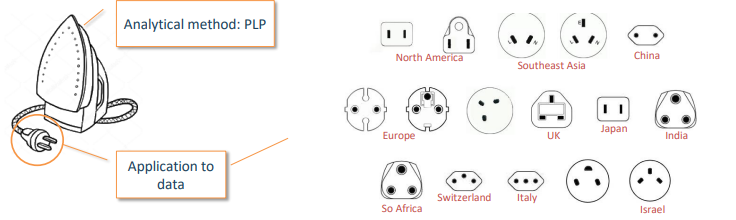
\includegraphics[width=0.60\textwidth]{figures/plancha1.png}
     %\caption{Ejemplo de la plancha con diferentes enchufes. Extraído de la web oficial \cite{OHDSIwebsite}}
    \label{fig:plancha1}
\end{figure}
\begin{figure}[H]
    \centering
    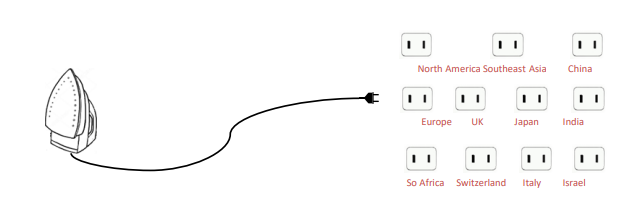
\includegraphics[width=0.70\textwidth]{figures/plancha2.png}
     \caption{Ejemplo de la plancha. Extraído de la web oficial \cite{OHDSIwebsite}}
    \label{fig:plancha2}
\end{figure}

    \item \textbf{Extracción de evidencia a partir de datos clínicos}. Es importante destacar la finalidad de OHDSI de, no solo recopilar y almacenar la información clínica, sino también extraer información o evidencia de ella. 
    %La organización identifica la dificultad de extraer información trascendental de los datos clíncos debido a sus distintas morfologías y estructuras en las que son recogidos. 
    Este es el propósito final y enfrenta muchos desafíos debido a la disparidad de los datos y técnicas de análisis. 
    
    El proceso de extracción de evidencia no es sencillo, como se muestra en la Figura \ref{fig:drawinJourney} ''Dibujo del proceso de extracción de evidencia'', y parte en un extremo de las diferentes bases de datos del mundo real (RWD) (véase \ref{sec:01Contexto} ''Marco contextual'') hacia la obtención fiable de evidencia del mundo real (RWE). Este recorrido debe atravesar un proceso de ETL para estandarizar las bases de datos al modelo común de OMOP, la integración con el vocabulario y el análisis técnico en sí que permita extraer la evidencia. Por suerte, la organización también proporciona un conjunto de herramientas (véase \ref{sec:05herramientas} ''Herramientas'') para realizar más sencillamente todo el recorrido.

\begin{figure}[H]
    \centering
    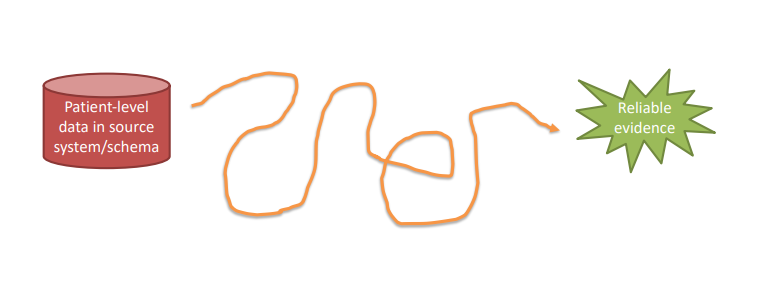
\includegraphics[width=0.80\textwidth]{figures/drawinJourney.png}
     \caption{Dibujo del proceso de extracción de evidencia. Extraído de la web oficial \cite{OHDSIwebsite}}
    \label{fig:drawinJourney}
\end{figure}



\end{enumerate}

%\section{Historia: Observational Medical Outcomes Partnership (OMOP)}

\section{¿Qué es OMOP?} \label{sec:05omop}

Es común encontrar en internet los términos OHDSI y OMOP (\textit{Observational Medical Outcomes Partnership}), utilizados de forma casi indistintiva. Si bien es verdad que OMOP se suele asociar mayoritariamente al CDM (\textit{Common Data Model}) también OHDSI mantiene gran relación con este modelo común de datos. Entonces, ¿cuál es la relación entre estas dos entidades? Pues bien, la iniciativa de OHDSI se originó en 2014, posterior al proyecto OMOP, que finalizó en 2013, pues la relación que guardan estas dos entidades es filial, OHDSI es la sucesora de OMOP. 

OMOP nació en 2008 como una asociación público-privada presidida por la Administración de Alimentos y Medicamentos de EE. UU. con el objetivo de establecer buenas prácticas en estudios observacionales retrospectivos. El proyecto además fue administrado por la Fundación de los Institutos Nacionales de Salud y financiado por un consorcio de compañías farmacéuticas en colaboración con otros investigadores académicos y socios de datos de salud \cite{stang2010advancing}. El propósito inicial de OMOP era impulsar la ciencia de la vigilancia activa de la seguridad de los productos médicos mediante el análisis de datos observacionales de atención médica \cite{stang2010advancing}. Sin embargo, durante su desarrollo, se enfrentó a los desafíos técnicos de llevar a cabo investigaciones en bases de datos observacionales muy heterogéneas entre sí.

El resultado fue el desarrollo de un Modelo Común de Datos (CDM) como un mecanismo para estandarizar la estructura, el contenido y la semántica de los datos observacionales y hacer posible escribir código de análisis estadístico que fuera reutilizable para estudios en distintas fuentes de datos \cite{overhage2012validation}. Los experimentos de OMOP demostraron la viabilidad de establecer un CDM que además reuniese diferentes vocabularios estandarizados, reuniendo en un mismo estándar diversos tipos de datos de diferentes entornos de atención y representados por diferentes vocabularios de origen. Esta característica facilitó la colaboración y aumentó el interés entre diferentes instituciones lo que promovió o un enfoque de ciencia abierta \cite{OHDSIbook}. OMOP puso todo su trabajo a disposición del público, incluidos diseños de estudio, estándares de datos, código de análisis y hallazgos empíricos, para mejorar la transparencia y fomentar la confianza en su investigación. 

Al término del proyecto, el Modelo Común de Datos (CDM) de OMOP había evolucionado hasta respaldar un abanico  amplísimo de aplicaciones analíticas, incluida la efectividad comparativa de intervenciones médicas y políticas de todo el sistema de salud, no solo de la industria farmacéutica, por tanto, el equipo de investigación acordó que el fin de dicho proyecto debería ser el origen de uno nuevo. a partir de esta idea nació OHDSI \cite{OHDSIbook}.

%\section{Actualidad de la organización}

Por tanto, lo que nació en 2014 como la continuación del proyecto OMOP ha evolucionado hasta convertirse en una extensa red colaborativa global.  En la actualidad, la comunidad de OHDSI cuenta con la participación de más de tres mil colaboradores distribuidos en 80 países.

\begin{figure}[H]
    \centering
    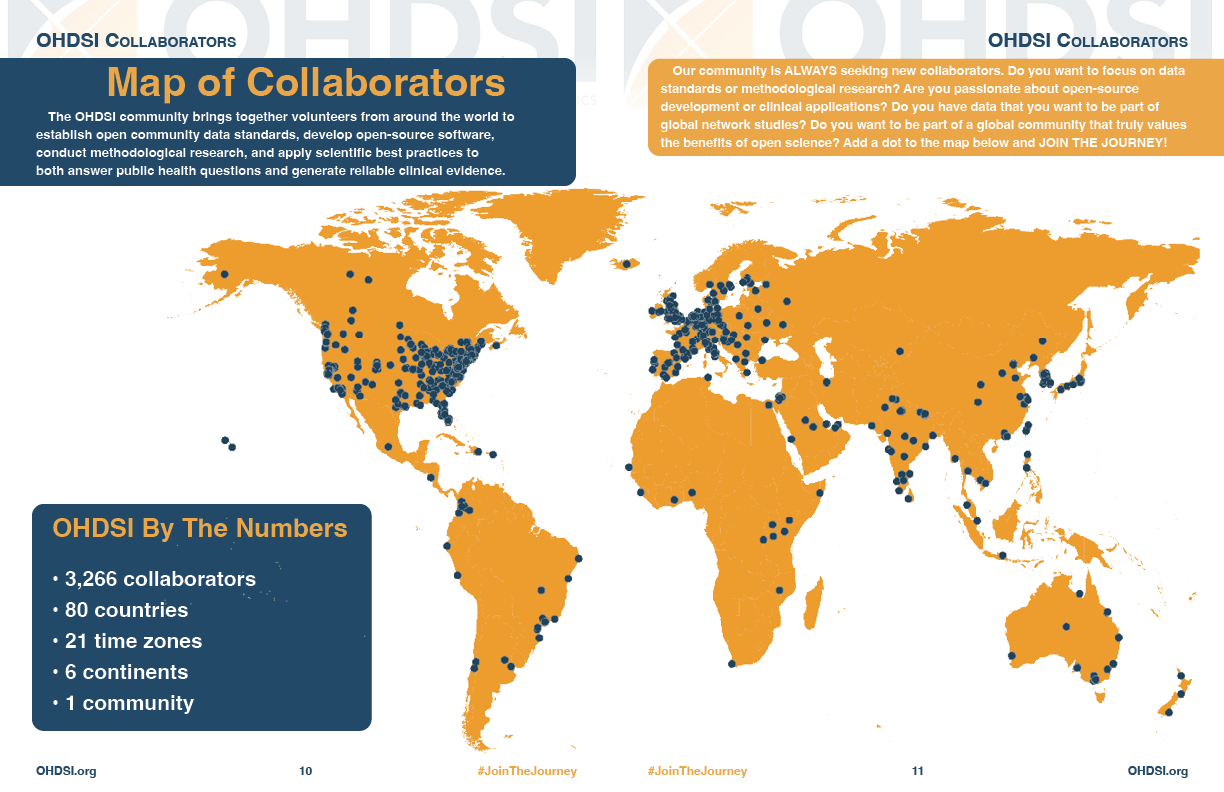
\includegraphics[width=0.80\textwidth]{figures/OHDSIcollaborators.png}
     \caption{Mapa de colaboradores de OHDSI. Extraído de la web oficial \cite{OHDSIwebsite}}
    \label{fig:OHDSIcollaborators}
\end{figure}

Además, tal y como se presenta en \ref{sec:01EstadoArte} ''Estado del arte'', desde que se inició su colaboración con EHDEN (European Health Data Evidence) en 2020, OHDSI está adquiriendo cada vez mayor relevancia a nivel europeo. Ejemplo de ello es la celebración, este mes de junio, en Rotterdam del quinto Symposium Europeo de OHDSI (véase Figura \ref{fig:bannerSymposyum2024} ''Banner del Symposium Europeo 2024''), que tiene el fin de reunir a los expertos y miembros de la comunidad para presentar los grandes proyectos nacionales y europeos que se están realizando en toda europa con las herramientas de la comunidad.

\begin{figure}[H]
    \centering
    
\includegraphics[width=0.70\textwidth]{figures/bannerSymposyum2024.jpg}
     \caption{Banner del Symposium Europeo 2024. Extraído de la web oficial \cite{OHDSIwebsite}}
    \label{fig:bannerSymposyum2024}
\end{figure}

Por ejemplo, en el Symposium Europeo del pasado año 2023, se presentaron proyectos relativos al almacenamiento de los datos de UCI en Holanda \cite{Jagesar2023The}, la integración del CDM de OMOP con el laboratorio de datos de salud alemám \cite{Finster2023Integrating}, la estandarización de la base de datos nacional francesa SNDS al modelo de OMOP \cite{Collumeau2023Standardization}, la armonización de los HCE hospitalarios en Ruanda al CDM \cite{Halvorsen2023Ruanda} y a la estandarización de los datos del registro europeo de sarcomas a OMOP \cite{vanSwieten2023Standardizing}, entre otros.

%La intención de esta sección es mostrar la gran relevancia que tiene actualmente la organización de OHDSI sobre todo en los grandes proyectos europeos. 

\section{¿Cómo generar evidencia?} \label{sec:05Evidencia}

Una vez que se conoce qué es OHDSI, su misión y sus características fundamentales, se conoce la importancia de generar evidencia a partir del estudio de los datos clínicos. A continuación se exponen los principios fundamentales de la organización para generar evidencia confiable.

\subsubsection{The journey from data to evidence}

No es casualidad que la invitación que hace OHDSI a sus colaboradores lleve el slogan \textit{''Join the Journey''} sino que es un guiño al propósito al que se unen, es decir, al camino desde los datos hasta la evidencia o, en ingles, \textit{"The Journey from data to evidence"}.

\begin{figure}[H]
    \centering
    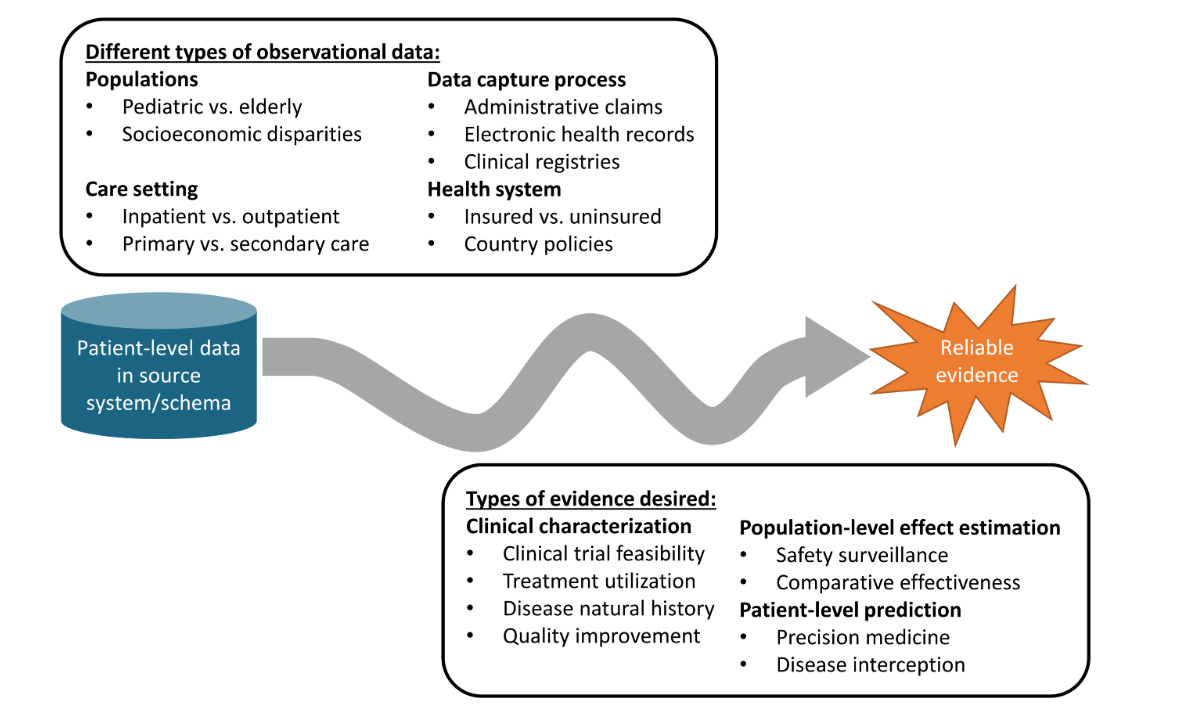
\includegraphics[width=0.80\textwidth]{figures/journeyDataToEvidence.png}
     \caption{\textit{The Journey from Data to Evidence}. Extraído del Libro de OHDSI \cite{OHDSIbook}}
    \label{fig:journeyDataToEvidence}
\end{figure}

La anterior Figura \ref{fig:journeyDataToEvidence} ''The Journey from Data to Evidence'' complementa a la Figura \ref{fig:drawinJourney} ''Dibujo del proceso de extracción de evidencia'' añadiendo mayor información sobre los diferentes tipos de datos que se recogen y los diferentes tipos de evidencia que se quiere generar. Frente a la disparidad de los datos y la finalidad con la que son recogidos, OHDSI presenta el Modelo de Datos Común (véase la subsección \ref{subsec:05cdm} ''Modelo de Datos Común'') y para la extracción de evidencia, la investigación metodológica mediante tres casos de uso fundamentales: la caracterización clínica de una cohorte, la estimación a nivel de población y la predicción a nivel de paciente (véase subsección \ref{subsec:05investMetodolog} ''Investigación metodológica'').

Los estudios que se llevan a cabo son \textbf{estudios observacionales o fenotípicos}, es decir, que simulan lo que sería un estudio clínico experimental sin intervención pero sobre datos ya almacenados de pacientes, en vez de realizar un seguimiento en vivo. De esta forma se logra obtener evidencia basada en datos. Cuando la evidencia se extrae sobre datos del mundo real (\textit{RWD}), se denomina evidencia del mundo real (\textit{Real World Evidence, RWE}).

%De esta forma, OHDSI promueve una vía para generar evidencia interoperable entre las distintas organizaciones que interactúan a través de su red mundial, dicho de otra forma, pretende dar soporte para que miles de estudios diferentes sigan una misma metodología que facilite su comprensión de forma global.

Además, una característica fundamental de las investigaciones que se llevan acabo en OHDSI es que giran entorno al paciente, que es además el núcleo central del Modelo de Datos Común de OMOP. Por lo que un componente fundamental de cualquier investigación metodológica son las historias de los pacientes. \textbf{Para cada evento clínico que sucede se recoge una historia del paciente o \textit{Patient Journey}}. Es importante no confundir este concepto con la Historia Clínica Electrónica de un paciente (HCE) que recoge una ficha con todos los eventos que han le sucedido a lo largo de su vida. Las investigaciones observacionales se diseñan para extraer información sobre la recopilación de todos los \textit{patient journeys}.

\begin{figure}[H]
    \centering
    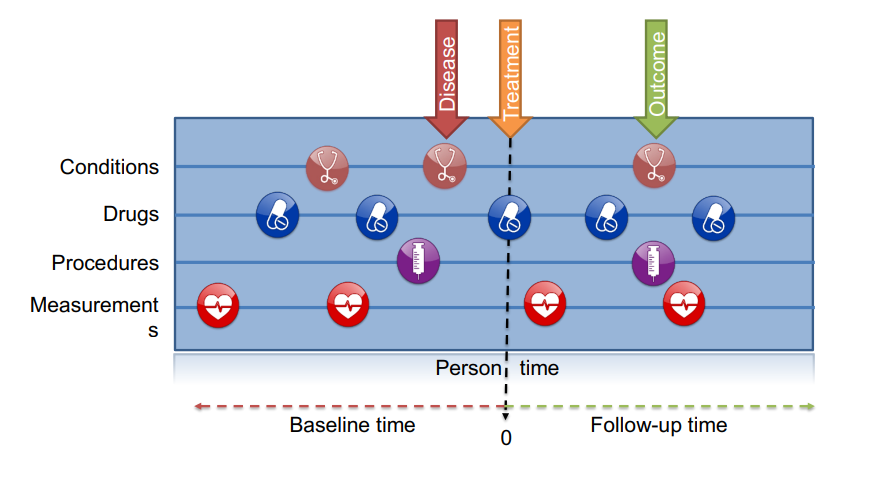
\includegraphics[width=0.80\textwidth]{figures/patientJourney.png}
     \caption{\textit{The patient journey}. Extraído de la página web oficial \cite{OHDSIbook}}
    \label{fig:patientJourney}
\end{figure}

La historia del paciente,  como se muestra en la Figura \ref{fig:patientJourney} ''The patient journey'', es por tanto, una ventana temporal que recoge un evento clínico que le sucede a un paciente en un período de tiempo concreto. El evento se describe mediante tres períodos de tiempo: la enfermedad (rojo), el tratamiento (naranja) y el efecto (verde); y a partir de cuatro características esenciales: síntomas (\textit{conditions}), medicamentos (\textit{drugs}), procedimientos (\textit{procedures}) y pruebas (\textit{measurements}).

Los pacientes se pueden agrupar en \textbf{cohortes} cuando comparten historias y características similares, al igual que a la hora de realizar un estudio clínico en vivo. Las diferentes  prácticas para los análisis de cohortes darán lugar a los diferentes tipos de evidencia deseada (caracterización, estimación a nivel de población, predicción a nivel de paciente). \textbf{Por tanto, el componente central para generar evidencia en OHDSI es la cohorte.}

%\begin{figure}[H]
%\centering
%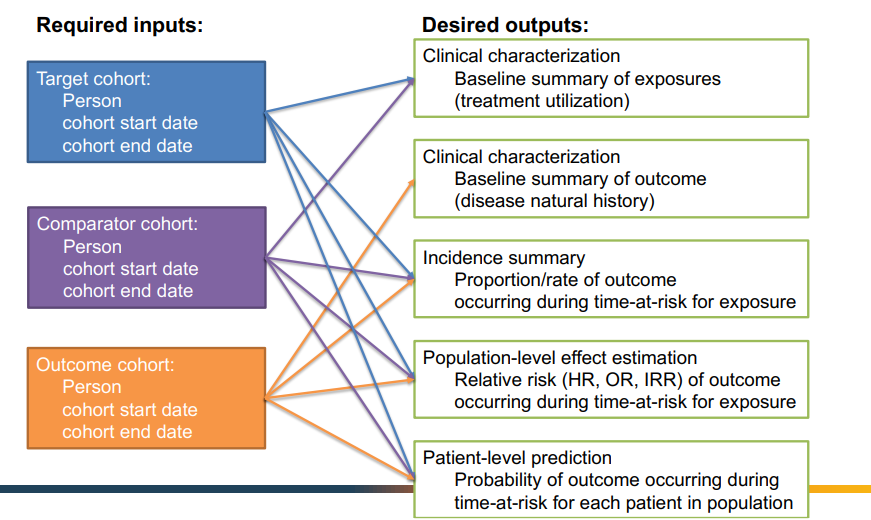
\includegraphics[width=0.70\textwidth]{figures/studyIO.png}
%     \caption{La definición de cohortes es el componente esencial para la generación de evidencia. Extraído del Tutorial2022 publicado en la web oficial \cite{OHDSIwebsite}}
%    \label{fig:studyIO}
%\end{figure}

\subsubsection{Implementación del análisis}

Para realizar un análisis, OHDSI distingue tres vías alternativas para generar la evidencia a partir de la base de datos estandarizada al OMOP CDM. Estas tres alternativas se muestran a continuación en la Figura \ref{fig:analysisImplementations} ''Tres vías para la implementación de un análisis observacional'', extraída del capítulo 8 del Libro de OHDSI.

\begin{figure}[H]
    \centering
    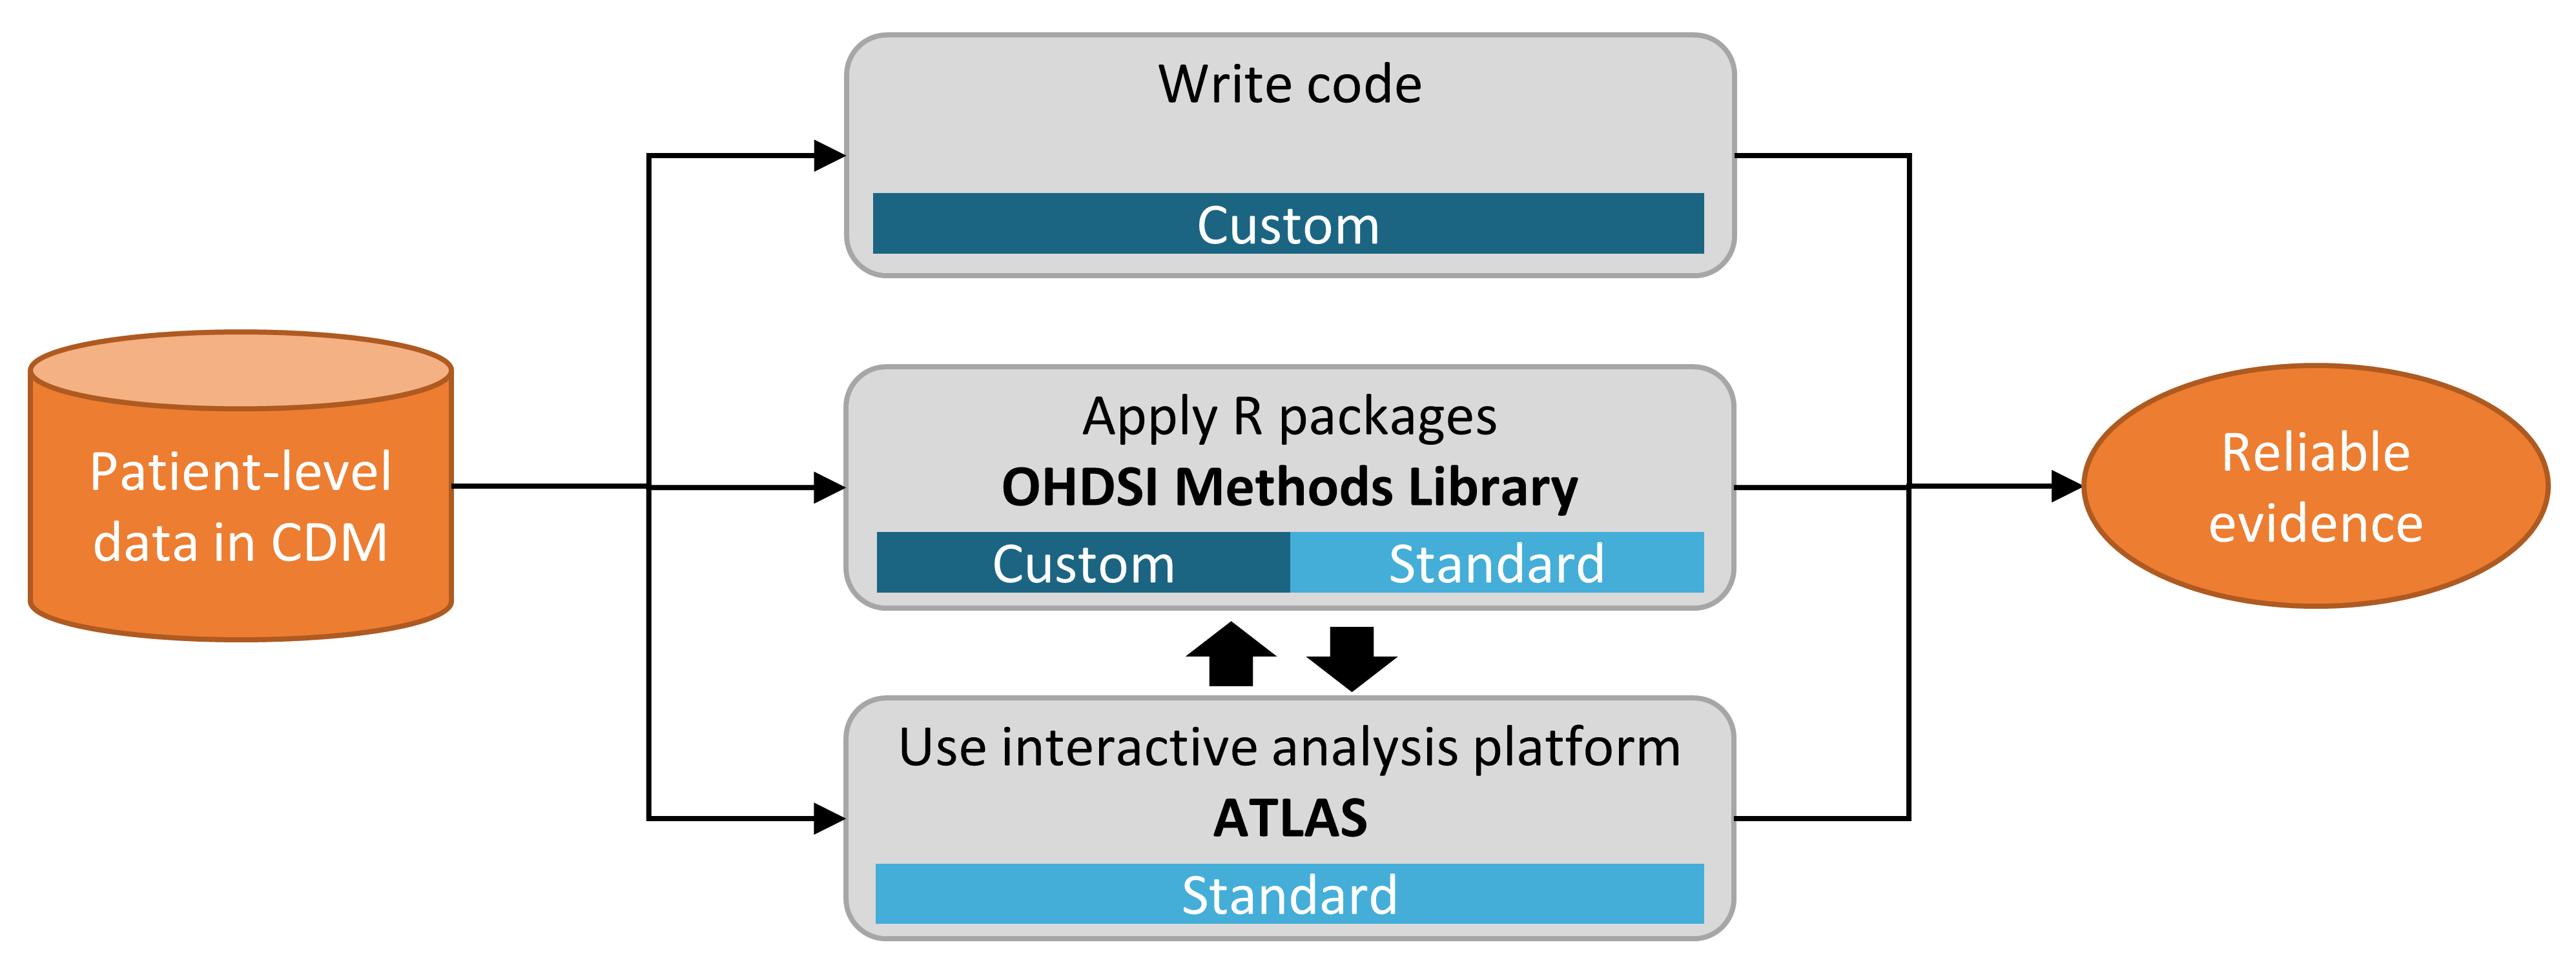
\includegraphics[width=0.80\textwidth]{figures/analysisImplementations.png}
     \caption{Tres vías para la implementación de un análisis observacional. Extraído del Libro de OHDSI \cite{OHDSIbook}}
    \label{fig:analysisImplementations}
\end{figure}

Cada vía se evalúa en cuanto a lo personalizada (\textit{custom}) o estandarizada (\textit{standard}) que es. A estas alturas se debe conocer que la vía más recomendada para implementar el análisis será la más estandarizada, es decir, la tercera vía.

La problemática que presentan la primera y la segunda vía consiste en ser en mayor o menor medida vías customizada, lo que genera problemas de interoperabilidad y reproducibilidad de los estudios. Si bien la primera vía consiste en la programación directa de código para realizar las consultas  (no hay ningún tipo de estandarización, distintos lenguajes de programación, funciones personalizadas) al menos la segunda vía hace uso de librerías estándares en R que OHDSI ofrece (\textit{OHDSI Methods Library}) pero, aunque se use el mismo lenguage de programación y funciones, los scripts pueden ser tan distintos que aún dificulten la interoperabilidad.

Por tanto, la tercera vía se presenta como la alternativa óptima por ser la más estandarizada y es la que empleará el TFG en el estudio práctico. Esto es, usar la herramienta interactiva \textit{low-code} de análisis de datos que ofrece OHDSI, denominada \textbf{ATLAS}, sin necesidad de programar directamente código.

\section{Conclusiones} \label{sec:05conclusion}

En este capítulo se concluye la relevancia de OHDSI en el panorama sanitario y tecnológico actual, capaz de subsanar las necesidades del mismo a través de su misión, estándares y herramientas.

Principalmente se realiza una labor importantísima de estandarización, tanto a nivel de datos mediante el Modelo de Datos Común y el Vocabulario como a nivel de estudios mediante la Investigación metodológica y sobre todo gracias al auge del uso de su herramienta estrella, ATLAS, que se emplea para el estudio práctico del TFG.